\documentclass[12pt, titlepage]{article}

\usepackage{fullpage}
\usepackage[round]{natbib}
\usepackage{multirow}
\usepackage{booktabs}
\usepackage{tabularx}
\usepackage{graphicx}
\usepackage{circuitikz}
\usepackage{float}
\usepackage{hyperref}
\hypersetup{
    colorlinks,
    citecolor=blue,
    filecolor=black,
    linkcolor=red,
    urlcolor=blue
}

%% Comments

\usepackage{color}

\newif\ifcomments\commentstrue %displays comments
%\newif\ifcomments\commentsfalse %so that comments do not display

\ifcomments
\newcommand{\authornote}[3]{\textcolor{#1}{[#3 ---#2]}}
\newcommand{\todo}[1]{\textcolor{red}{[TODO: #1]}}
\else
\newcommand{\authornote}[3]{}
\newcommand{\todo}[1]{}
\fi

\newcommand{\wss}[1]{\authornote{blue}{SS}{#1}} 
\newcommand{\plt}[1]{\authornote{magenta}{TPLT}{#1}} %For explanation of the template
\newcommand{\an}[1]{\authornote{cyan}{Author}{#1}}

%% Common Parts

\newcommand{\progname}{Natural Language Processing for Mental Health Risk Prediction} % PUT YOUR PROGRAM NAME HERE
\newcommand{\authname}{Team 13, The Cognitive Care Crew
\\ Jessica Dawson
\\ Michael Breau
\\ Matthew Curtis
\\ Benjamin Chinnery
\\ Yaruo Tian} % AUTHOR NAMES                  

\usepackage{hyperref}
    \hypersetup{colorlinks=true, linkcolor=blue, citecolor=blue, filecolor=blue,
                urlcolor=blue, unicode=false}
    \urlstyle{same}
                                


\newcounter{acnum}
\newcommand{\actheacnum}{AC\theacnum}
\newcommand{\acref}[1]{AC\ref{#1}}

\newcounter{ucnum}
\newcommand{\uctheucnum}{UC\theucnum}
\newcommand{\uref}[1]{UC\ref{#1}}

\newcounter{mnum}
\newcommand{\mthemnum}{M\themnum}
\newcommand{\mref}[1]{M\ref{#1}}

\newcounter{edmnum}
\newcommand{\edmthemnum}{EDM\theedmnum}
\newcommand{\edmref}[1]{EDM\ref{#1}}

\setcounter{secnumdepth}{5}

\graphicspath{ {./figs/} }

\begin{document}

\title{Module Guide for \progname{}} 
\author{\authname}
\date{\today}

\maketitle

\pagenumbering{roman}

\section{Revision History}

\begin{tabularx}{\textwidth}{p{3cm}p{2cm}X}
\toprule {\bf Date} & {\bf Version} & {\bf Notes}\\
\midrule
January 17, 2024 & 1.0 & Revision 0\\
\bottomrule
\end{tabularx}

\newpage

\section{Reference Material}

This section records information for easy reference.

\subsection{Abbreviations and Acronyms}

\renewcommand{\arraystretch}{1.2}
\begin{tabular}{l l} 
  \toprule		
  \textbf{symbol} & \textbf{description}\\
  \midrule 
  AC & Anticipated Change\\
  ED & Eating Disorder\\
  DAG & Directed Acyclic Graph \\
  M & Module \\
  MG & Module Guide \\
  OS & Operating System \\
  R & Requirement\\
  SC & Scientific Computing \\
  SRS & Software Requirements Specification\\
  UC & Unlikely Change \\
  \bottomrule
\end{tabular}\\

\newpage

\tableofcontents

\listoftables

\listoffigures

\newpage

\pagenumbering{arabic}

\section{Introduction}

Decomposing a system into modules is a commonly accepted approach to developing
software.  A module is a work assignment for a programmer or programming
team~\citep{ParnasEtAl1984}.  We advocate a decomposition
based on the principle of information hiding~\citep{Parnas1972a}.  This
principle supports design for change, because the ``secrets'' that each module
hides represent likely future changes.  Design for change is valuable in SC,
where modifications are frequent, especially during initial development as the
solution space is explored.  

Our design follows the rules layed out by \citet{ParnasEtAl1984}, as follows:
\begin{itemize}
\item System details that are likely to change independently should be the
  secrets of separate modules.
\item Each data structure is implemented in only one module.
\item Any other program that requires information stored in a module's data
  structures must obtain it by calling access programs belonging to that module.
\end{itemize}

After completing the first stage of the design, the Software Requirements
Specification (SRS), the Module Guide (MG) is developed~\citep{ParnasEtAl1984}. The MG
specifies the modular structure of the system and is intended to allow both
designers and maintainers to easily identify the parts of the software.  The
potential readers of this document are as follows:

\begin{itemize}
\item New project members: This document can be a guide for a new project member
  to easily understand the overall structure and quickly find the
  relevant modules they are searching for.
\item Maintainers: The hierarchical structure of the module guide improves the
  maintainers' understanding when they need to make changes to the system. It is
  important for a maintainer to update the relevant sections of the document
  after changes have been made.
\item Designers: Once the module guide has been written, it can be used to
  check for consistency, feasibility, and flexibility. Designers can verify the
  system in various ways, such as consistency among modules, feasibility of the
  decomposition, and flexibility of the design.
\end{itemize}

The rest of the document is organized as follows. Section
\ref{SecChange} lists the anticipated and unlikely changes of the software
requirements. Section \ref{SecMH} summarizes the module decomposition that
was constructed according to the likely changes. Section \ref{SecConnection}
specifies the connections between the software requirements and the
modules. Section \ref{SecMD} gives a detailed description of the
modules. Section \ref{SecTM} includes two traceability matrices. One checks
the completeness of the design against the requirements provided in the SRS. The
other shows the relation between anticipated changes and the modules. Section
\ref{SecUse} describes the use relation between modules.

\section{General Structure of an NLP Pipeline} \label{SecPipeline}

All NLP pipelines in this system can be thought of as following a general structure. This is not a hard description of the structure each diagnosis component will use but a soft description of what the system's NLP pipelines will look like. This pattern is likely to show up throughout the system in various locations and is included here to provide context and a conceptual model the reader can use for the rest of the document. The proposed structure is as follows: \newline

\noindent Input $\rightarrow$ Tokenizer $\rightarrow$ Representation Model $\rightarrow$ Prediction Model $\rightarrow$ Predictions \newline

\noindent Where the Prediciton Model can be further broken up into: \newline

\noindent $\rightarrow$ Transformation $\rightarrow$ ... $\rightarrow$ Transformation $\rightarrow$ \newline

\noindent A brief description of each stage is as follows:

\begin{itemize}
    \item Input: The input text to the pipeline.
    \item Tokenizer: Responsible for "cleaning" the text, can perform many different tasks: removing junk words (often referred to as stopwords) like the, and, a, etc.; expanding contractions; removing numerics and URLS. Leaves the text as text, just with the less useful features removed.
    \item Representation Model: Machine learning models can not directly operate on text, they need numerical inputs. The representation model converts from the text to some numerical format, typically a vector. Different representation models output different formats and encode different information into these formats.
    \item Prediction Model: Transforms the numerical format provided by the representation model into the mental health predictions of interest. The prediction model may transform the data mutliple times in different ways before reaching a final prediction.
    \begin{itemize}
        \item Transformation: A specific transformation in the prediction model's pipeline
    \end{itemize}
    \item Predictions: The final predictions produced by the pipeline.
\end{itemize}

Due to the interconnected nature of this pipeline and the research based nature of this project large changes to the system's models are both expected and unavoidable. This is because changes in one section of pipeline can require large changes in other sections, trying a new prediction model may require an entirely different representation model to be used for example.

\section{Anticipated and Unlikely Changes} \label{SecChange}

This section lists possible changes to the system. According to the likeliness
of the change, the possible changes are classified into two
categories. Anticipated changes are listed in Section \ref{SecAchange}, and
unlikely changes are listed in Section \ref{SecUchange}.

\subsection{Anticipated Changes} \label{SecAchange}

Anticipated changes are the source of the information that is to be hidden
inside the modules. Ideally, changing one of the anticipated changes will only
require changing the one module that hides the associated decision. The approach
adapted here is called design for
change.

\begin{description}
\item[\refstepcounter{acnum} \actheacnum \label{acInput}:] What format the input data takes.
\item[\refstepcounter{acnum} \actheacnum \label{acOutput}:] What format the output data takes.
\item[\refstepcounter{acnum} \actheacnum \label{acData}:] In what format the data is stored during runtime. Different layouts can change how quickly certain information can be accessed and effect performance.
\item[\refstepcounter{acnum} \actheacnum \label{acPipelineStages}:] What stages there are in a task's NLP pipeline.
\item[\refstepcounter{acnum} \actheacnum \label{acTokenization}:] How the raw text data is "cleaned" (see \ref{SecPipeline}: tokenizer).
\item[\refstepcounter{acnum} \actheacnum \label{acRepModel}:] How the cleaned text data is converted into numerical data.
\item[\refstepcounter{acnum} \actheacnum \label{acPredModel}:] How many manipulations of the numerical data are performed before producing a prediction.
\item[\refstepcounter{acnum} \actheacnum \label{acTrans}:] How the numerical data is manipulated to produce predictions.
\item[\refstepcounter{acnum} \actheacnum \label{acParams}:] What the optimal parameters for a pipeline will be.
\item[\refstepcounter{acnum} \actheacnum \label{acMets}:] How the accuracy of a pipeline will be evaluated.
\item[\refstepcounter{acnum} \actheacnum \label{acOps}:] How the system will integrate with the tools the operations team is developing.
\end{description}

\subsection{Unlikely Changes} \label{SecUchange}

The module design should be as general as possible. However, a general system is
more complex. Sometimes this complexity is not necessary. Fixing some design
decisions at the system architecture stage can simplify the software design. If
these decision should later need to be changed, then many parts of the design
will potentially need to be modified. Hence, it is not intended that these
decisions will be changed.

\begin{description}
\item[\refstepcounter{ucnum} \uctheucnum \label{ucIO}:] Input/Output devices
  (Input: File, Output: File).
\item[\refstepcounter{ucnum} \uctheucnum \label{ucTasks}:] What diagnosis tools the system will provide.
\end{description}

\section{Module Hierarchy} \label{SecMH}

This section provides an overview of the module design. Modules are summarized
in a hierarchy decomposed by secrets in Table \ref{TblMH}. The modules listed
below, which are leaves in the hierarchy tree, are the modules that will
actually be implemented:
\begin{description}
\item [\refstepcounter{mnum} \mthemnum \label{mHH}:] Hardware-Hiding Module
\item [\refstepcounter{mnum} \mthemnum \label{DNOM1}:] Depression Main Module
\item [\refstepcounter{mnum} \mthemnum \label{DNOM2}:] Depression Data Processing Module
\item [\refstepcounter{mnum} \mthemnum \label{DNOM3}:] Depression Feature Extraction Module
\item [\refstepcounter{mnum} \mthemnum \label{DNOM4}:] Depression Output Module
\item [\refstepcounter{mnum} \mthemnum \label{DNOM5}:] Depression Evaluation Module
\item [\refstepcounter{mnum} \mthemnum \label{ANOM1}:] Anorexia Main Module
\item [\refstepcounter{mnum} \mthemnum \label{ANOM2}:] Anorexia Parser Module
\item [\refstepcounter{mnum} \mthemnum \label{ANOM3}:] Anorexia Training Module
\item [\refstepcounter{mnum} \mthemnum \label{ANOM4}:] Anorexia Predictor Module
\item [\refstepcounter{edmnum} \edmthemnum \label{edmPars}:] ED Parsing
\item [\refstepcounter{edmnum} \edmthemnum \label{edmClean}:] ED Cleaning
\item [\refstepcounter{edmnum} \edmthemnum \label{edmO}:] ED Output
\item [\refstepcounter{edmnum} \edmthemnum \label{edmPipeline}:] ED Pipeline Manager
\item [\refstepcounter{edmnum} \edmthemnum \label{edmTr}:] ED Trainer
\item [\refstepcounter{edmnum} \edmthemnum \label{edmData}:] ED Data Storage
\item [\refstepcounter{edmnum} \edmthemnum \label{edmRM}:] ED Representation Model
\item [\refstepcounter{edmnum} \edmthemnum \label{edmRel}:] ED Relabeler
\item [\refstepcounter{edmnum} \edmthemnum \label{edmPM}:] ED Prediction Model
\item [\refstepcounter{edmnum} \edmthemnum \label{edmAgg}:] ED Aggregator
\item [\refstepcounter{edmnum} \edmthemnum \label{edmMets}:] ED Metrics
\item [\refstepcounter{edmnum} \edmthemnum \label{edmEval}:] ED Evaluator
\item [\refstepcounter{edmnum} \edmthemnum \label{edmViz}:] ED Visualization
\end{description}


\begin{table}[H]
\centering
\begin{tabular}{p{0.2\textwidth} p{0.3\textwidth} p{0.4\textwidth}}
\toprule
\textbf{Level 1} & \textbf{Level 2} & \textbf{Level 3}\\
\midrule

{Hardware-Hiding} & None \\
\midrule

\multirow{3}{*}{Behaviour-Hiding} & \\ \cline{2-3}
& \multirow{2}{*}{Eating Disorder IO} & ED Input\\
& & ED Output\\
\midrule

\multirow{16}{*}{Software Decision} 
& \multirow{5}{*}{Depression Pipeline} & Depression Main\\ 
& & Depression Data Processing\\
& & Depression Feature Extraction\\
& & Depression Output\\ 
& & Depression Evaluation\\\cline{2-3}
& \multirow{4}{*}{Anorexia Pipeline} & Anorexia Main\\ 
& & Anorexia Parser\\
& & Anorexia Training\\
& & Anorexia Predictor\\ \cline{2-3}
& \multirow{7}{*}{Eating Disorder Pipeline} & ED Pipeline Manager\\
& & ED Trainer\\
& & ED Data Storage\\
& & ED Representation Model\\
& & ED Relabeler\\
& & ED Prediction Model\\
& & ED Aggregator\\
& & ED Evaluation\\
\bottomrule

\end{tabular}
\caption{Module Hierarchy}
\label{TblMH}
\end{table} \newpage

\begin{table}[H]
\centering
\begin{tabular}{p{0.5\textwidth} p{0.5\textwidth}}
\toprule
\textbf{Level 3} & \textbf{Level 4}\\

\midrule
\multirow{2}{*}{ED Input} & ED Parsing\\
& ED Cleaning\\ \midrule
ED Output &\\
\midrule

Depression Main &\\ 
Depression Data Processing &\\
Depression Feature Extraction &\\
Depression Output &\\ 
Depression Evaluation &\\ \midrule
Anorexia Main &\\ 
Anorexia Parser &\\
Anorexia Training &\\
Anorexia Predictor &\\ \midrule
ED Pipeline Manager &\\
ED Trainer &\\
ED Data Storage &\\
ED Representation Model &\\
ED Relabeler &\\
ED Prediction Model &\\
ED Aggregator &\\ \midrule
\multirow{3}{*}{ED Evaluation} & ED Metrics\\
& ED Evaluator\\
& ED Visualization\\

\bottomrule

\end{tabular}
\caption{Module Hierarchy cont}
\label{TblMH2}
\end{table}

\newpage

\section{Connection Between Requirements and Design} \label{SecConnection}

The design of the system is intended to satisfy the requirements developed in
the SRS. In this stage, the system is decomposed into modules. The connection
between requirements and modules is listed in Table~\ref{TblRT}.

\section{Module Decomposition} \label{SecMD}

Modules are decomposed according to the principle of ``information hiding''
proposed by \citet{ParnasEtAl1984}. The \emph{Secrets} field in a module
decomposition is a brief statement of the design decision hidden by the
module. The \emph{Services} field specifies \emph{what} the module will do
without documenting \emph{how} to do it. For each module, a suggestion for the
implementing software is given under the \emph{Implemented By} title. If the
entry is \emph{OS}, this means that the module is provided by the operating
system or by standard programming language libraries.

Only the leaf modules in the hierarchy have to be implemented. If a dash
(\emph{--}) is shown, this means that the module is not a leaf and will not have
to be implemented.

\subsection{Hardware Hiding Modules (\mref{mHH})}

\begin{description}
\item[Secrets:]The data structure and algorithm used to implement the virtual
  hardware.
\item[Services:]Serves as a virtual hardware used by the rest of the
  system. This module provides the interface between the hardware and the
  software. So, the system can use it to display outputs or to accept inputs.
\item[Implemented By:] OS
\end{description}

\subsection{Behaviour-Hiding Module}

\begin{description}
\item[Secrets:]The contents of the required behaviours.
\item[Services:]Includes programs that provide externally visible behaviour of
  the system as specified in the software requirements specification (SRS)
  documents. This module serves as a communication layer between the
  hardware-hiding module and the software decision module. The programs in this
  module will need to change if there are changes in the SRS.
\item[Implemented By:] Depression IO, Anorexia IO, Eating Disorder IO
\end{description}

\subsubsection{Eating Disorder IO (-)}
\begin{description}
\item[Secrets:]How input and output is handled for the eating disorder diagnosis tool.
\item[Services:]Includes programs that provide reading from an input file and outputting to an output file for the eating disorder diagnosis tool.
\item[Implemented By:] ED Input, ED Output
\end{description}

\paragraph{ED Input (-)}
\begin{description}
\item[Secrets:] What format the input file is provided in.
\item[Services:] Provides functionality for reading user posts from a file and formatting them into a data structure usable by the rest of the system.
\item[Implemented By:] ED Parsing, ED Cleaning
\end{description}

\paragraph{ED Parsing (\edmref{edmPars})}
\begin{description}
\item[Secrets:] What format the input file is provided in.
\item[Services:] Provides functionality for reading user posts from a file.
\item[Implemented By:] parsing code developed for this project
\item[Type of Module:] Library
\end{description}

\paragraph{ED Cleaning (\edmref{edmClean})}
\begin{description}
\item[Secrets:] What the initial fields and structure of the data is.
\item[Services:] Cleans the data into a form ready to be used by the rest of the pipeline..
\item[Implemented By:] cleaning code developed for this project
\item[Type of Module:] Library
\end{description}

\paragraph{ED Output (\edmref{edmO})}
\begin{description}
\item[Secrets:]What format the output file is written in.
\item[Services:] Provides functionality for writing predictions to a file.
\item[Implemented By:] ED output code
\item[Type of Module:] Library
\end{description}

\subsection{Software Decision Module}
\subsubsection{Depression Main Module (\mref{DNOM1})}
\begin{description}
\item[Secrets:]The Natural Language processor which will combine the depression related functions such as process data, extract features, generating output, and evaluation to compute symptoms of depression in new documents.
\item[Services:] Depression training data do not provide direct interaction with the user. 
\item[Implemented By:] task1\_main
\end{description}

\subsubsection{Depression Data Processing Module (\mref{DNOM2})}
\begin{description}
\item[Secrets:]The parser for taking user posts and converting them into a format readable by the nlp model.
\item[Services:] Depresson training data do not provide direct interaction with the user. 
\item[Implemented By:] task1\_DataProcessing
\end{description}

\subsubsection{Depression Feature Extraction Module (\mref{DNOM3})}
\begin{description}
\item[Secrets:]The Natural Language processor which will analyze, compute with NLP techniques and extract the necessary features on parsed data.
\item[Services:] Depression training data do not provide direct interaction with the user. 
\item[Implemented By:] task1\_FeatureExtraction
\end{description}

\subsubsection{Depression Output Module (\mref{DNOM4})}
\begin{description}
\item[Secrets:]The Natural Language processor which will take the extracted features and generate sentences that shows symptoms of depression.
\item[Services:] Depression training data do not provide direct interaction with the user. 
\item[Implemented By:] task1\_Output
\end{description}

\subsubsection{Depression Evaluation Module (\mref{DNOM5})}
\begin{description}
\item[Secrets:]The Natural Language processor which will evaluate the output generated by measuring it against various metrics.
\item[Services:] Depression training data do not provide direct interaction with the user. 
\item[Implemented By:] task1\_Evaluation
\end{description}

\subsubsection{Anorexia Main Module (\mref{ANOM1})}
\begin{description}
\item[Secrets:] The Natural Language processor which will combine the parser, training, and predictor modules to compute anorexia risk in new documents.
\item[Services:] Anorexia training data
  do not provide direct interaction with the user. 
\item[Implemented By:] task2\_main
\end{description}

\subsubsection{Anorexia Parser Module (\mref{ANOM2})}
\begin{description}
\item[Secrets:] The parser for taking user posts and converting them into a format readable by the nlp model.
\item[Services:] Anorexia training data
  do not provide direct interaction with the user. 
\item[Implemented By:] task2\_parser
\end{description}

\subsubsection{Anorexia Training Module (\mref{ANOM3})}
\begin{description}
\item[Secrets:] The Natural Language processor which will train the model on parsed data.
\item[Services:] Anorexia training data
  do not provide direct interaction with the user. 
\item[Implemented By:] task2\_training
\end{description}

\subsubsection{Anorexia Predictor Module (\mref{ANOM4})}
\begin{description}
\item[Secrets:] The Natural Language processor which will analyze inputted user data to determine a risk for anorexia
\item[Services:] Anorexia training data
  do not provide direct interaction with the user. 
\item[Implemented By:] task2\_predictor
\end{description}

\subsubsection{Eating Disorder Pipeline (-)}
\begin{description}
\item[Secrets:] The structure and design of the eating disorder NLP pipeline.
\item[Services:] Includes programs that manage the overall pipeline and others that define the specific transformations used to produce a prediction. More details on the structure of the pipeline and how modules fit together can be found in section \ref{SecUse}.
\item[Implemented By:] ED Pipeline Manager, ED Representation Model, ED Relabeler, ED Aggregator ED Prediction Model, ED Trainer, ED Evaluator
\end{description}

\paragraph{ED Pipeline Manager (\edmref{edmPipeline})}
\begin{description}
\item[Secrets:] What components the NLP pipeline for the eating disorder task is comprised of.
\item[Services:] Orchestrates and runs all the components of the eating disorder NLP pipeline when used for predicting a score.
\item[Implemented By:] pipeline manager code developed for the project
\item[Type of Module:] Library
\end{description}

\paragraph{ED Trainer (\edmref{edmTr})}
\begin{description}
\item[Secrets:] How the pipeline is optimized and tuned.
\item[Services:] Orchestrates the tuning of models and model parameters for the pipeline.
\item[Implemented By:] trainer code developed for the project
\item[Type of Module:] Library
\end{description}

\paragraph{ED Data Storage (\edmref{edmData})}
\begin{description}
\item[Secrets:] What format the data is stored in during runtime.
\item[Services:] Abstracts away the underlying data format and provides an interface for accessing features of the data.
\item[Implemented By:] data storage code developed for the project
\item[Type of Module:] ADT
\end{description}

\paragraph{ED Representation Model (\edmref{edmRM})}
\begin{description}
\item[Secrets:] How text data is converted into a numerical format.
\item[Services:] Provides a routine for converting text data into a numerical format.
\item[Implemented By:] representation model code developed for the project
\item[Type of Module:] Library
\end{description}

\paragraph{ED Relabeler (\edmref{edmRel})}
\begin{description}
\item[Secrets:] How scores for each user in the ED data are converted into scores for each post.
\item[Services:] Provides a tool for creating scores for each post in the ED data based on the scores for each user. For more details on how this relabeling is used see section \ref{SecUse}
\item[Implemented By:] relabeling code developed for the project
\item[Type of Module:] ADT
\end{description}

\paragraph{ED Prediction Model (\edmref{edmPM})}
\begin{description}
\item[Secrets:] How the numerical representation of text from the Representation Model is converted to predictions.
\item[Services:] Orchestrates and runs all the transformations that make up the prediction model.
\item[Implemented By:] prediction model code developed for the project
\item[Type of Module:] ADT
\end{description}

\paragraph{ED Aggregator (\edmref{edmAgg})}
\begin{description}
\item[Secrets:] How scores for each post in a user's post history are converted to a single score for the user.
\item[Services:] Provides a tool for creating a single score for a user from scores for each of their posts.
\item[Implemented By:] aggregation code developed for the project
\item[Type of Module:] ADT
\end{description}

\paragraph{ED Evaluation (-)}
\begin{description}
\item[Secrets:] How the accuracy of model will be evaluated.
\item[Services:] Provides functions and routines for evaluating on specific metrics against certain baselines, and visualizing the data.
\item[Implemented By:] ED Metrics, ED Evaluator, ED Visualization
\end{description}

\paragraph{ED Metrics (\edmref{edmMets})}
\begin{description}
\item[Secrets:] What accuracy measures the model will be evaluated on.
\item[Services:] Provides functions for evaluating predictions on different metrics.
\item[Implemented By:] metrics code written for this project
\item[Type of Module:] Library
\end{description}

\paragraph{ED Evaluator (\edmref{edmEval})}
\begin{description}
\item[Secrets:] What baselines a model will be evaluated against.
\item[Services:] Provides functions for seeing the performance of baselines as compared to a model.
\item[Implemented By:] evaluator code written for this project
\item[Type of Module:] ADT
\end{description}

\paragraph{ED Visualization (\edmref{edmViz})}
\begin{description}
\item[Secrets:] What methods there are to visualize the data.
\item[Services:] Provides functions for visualizing different aspects of the data through graphs and plots.
\item[Implemented By:] visualization code written for this project
\item[Type of Module:] Library
\end{description}


\section{Traceability Matrix} \label{SecTM}

This section shows two traceability matrices: between the modules and the
requirements and between the modules and the anticipated changes.

% the table should use mref, the requirements should be named, use something
% like fref
\begin{table}[H]
\centering
\begin{tabular}{p{0.2\textwidth} p{0.6\textwidth}}
\toprule
\textbf{Req.} & \textbf{Modules}\\
\midrule
T1FR-1 & \mref{DNOM1}, \mref{DNOM2}\\
T1FR-2 & \mref{DNOM1}, \mref{DNOM3}\\
T1FR-3 & \mref{DNOM1}, \mref{DNOM4}, \mref{DNOM5}\\
T2FR-1 & \mref{ANOM1}, \mref{ANOM2}\\
T2FR-2 & \mref{ANOM1}, \mref{ANOM4}\\
T2FR-3 & \mref{ANOM1}, \mref{ANOM3}, \mref{ANOM4}\\
T2FR-4 & \mref{ANOM1}, \mref{ANOM4}\\
T3FR-1 & \edmref{edmPars}, \edmref{edmClean}\\
T3FR-2 & \edmref{edmO}\\
T3FR-3 & \edmref{edmO}\\
T3FR-4 & \edmref{edmPipeline}, \edmref{edmTr}, \edmref{edmRM}, \edmref{edmRel}, \edmref{edmPM}, \edmref{edmAgg}, \edmref{edmMets}, \edmref{edmEval}, \edmref{edmViz}\\
T3FR-5 & \edmref{edmPipeline}, \edmref{edmTr}, \edmref{edmRM}, \edmref{edmRel}, \edmref{edmPM}, \edmref{edmAgg}, \edmref{edmMets}, \edmref{edmEval}, \edmref{edmViz}\\
T3FR-6 & \edmref{edmPipeline}, \edmref{edmTr}, \edmref{edmRM}, \edmref{edmRel}, \edmref{edmPM}, \edmref{edmAgg}, \edmref{edmMets}, \edmref{edmEval}, \edmref{edmViz}\\
GR1 & \mref{DNOM1}, \mref{ANOM1}, \edmref{edmPars}, \edmref{edmO}\\
GR2 & \mref{DNOM4}, \mref{ANOM4}, \edmref{edmO}\\
SR1 & \mref{DNOM1}, \mref{ANOM1}, \edmref{edmO}\\
SR2 & \mref{DNOM4}, \mref{ANOM4}, \edmref{edmO}\\

\bottomrule
\end{tabular}
\caption{Trace Between Requirements and Modules}
\label{TblRT}
\end{table}

\begin{table}[H]
\centering
\begin{tabular}{p{0.2\textwidth} p{0.6\textwidth}}
\toprule
\textbf{AC} & \textbf{Modules}\\
\midrule
\acref{acInput} & \mref{DNOM2}, \mref{ANOM2}, \edmref{edmPars}\\
\acref{acOutput} & \mref{DNOM4}, \mref{ANOM4}, \edmref{edmO}\\
\acref{acData} & \edmref{edmData}\\
\acref{acPipelineStages} & \mref{DNOM1}, \mref{ANOM1}, \edmref{edmPipeline}\\
\acref{acTokenization} & \mref{DNOM2}, \mref{ANOM2}, \edmref{edmClean}, \edmref{edmRM}\\
\acref{acRepModel} & \mref{DNOM3}, \mref{ANOM3}, \edmref{edmRM}\\
\acref{acPredModel} & \mref{DNOM3}, \mref{ANOM3}, \edmref{edmRel}, \edmref{edmPM}, \edmref{edmAgg}\\
\acref{acTrans} & \mref{DNOM3}, \mref{ANOM4}, \edmref{edmRel}, \edmref{edmPM}, \edmref{edmAgg}\\
\acref{acParams} & \mref{DNOM1}, \mref{ANOM3}, \edmref{edmTr}\\
\acref{acMets} & \mref{DNOM5}, \mref{ANOM4}, \edmref{edmMets}, \edmref{edmEval}, \edmref{edmViz}\\
\acref{acOps} & \mref{DNOM1}, \mref{ANOM1}, \edmref{edmPipeline}\\

\bottomrule
\end{tabular}
\caption{Trace Between Anticipated Changes and Modules}
\label{TblACT}
\end{table}

\section{Pipeline Structure and Use Hierarchy Between Modules} \label{SecUse}

%In this section, the uses hierarchy between modules is
%provided. \citet{Parnas1978} said of two programs A and B that A {\em uses} B if
%correct execution of B may be necessary for A to complete the task described in
%its specification. That is, A {\em uses} B if there exist situations in which
%the correct functioning of A depends upon the availability of a correct
%implementation of B.  Figure \ref{FigUH} illustrates the use relation between
%the modules. It can be seen that the graph is a directed acyclic graph
%(DAG). Each level of the hierarchy offers a testable and usable subset of the
%system, and modules in the higher level of the hierarchy are essentially simpler
%because they use modules from the lower levels.

\subsection{Depression}

The pipeline for the depression module has \mref{DNOM1} Depression Main orchestrating the different stages. \mref{DNOM2} Data Processing processes the input data and converts to a usable form. \mref{DNOM3} Feature Extraction then pulls the most important features out of this data and feeds it to \mref{DNOM4} which writes to an output. \mref{DNOM5} provides evaluation metrics so the developer can see the accuracy of the model.

\begin{figure}[H]
\centering
\resizebox{0.7\textwidth}{!}{%
\begin{circuitikz}
\tikzstyle{every node}=[font=\normalsize]
\draw  (3,12.5) rectangle  node {\normalsize Processing} (7,11.5);
\draw  (8.75,15.75) rectangle  node {\normalsize Main} (12,14.75);
\draw  (8.5,12.5) rectangle  node {\normalsize Feature Extraction} (12.5,11.5);
\draw  (13.75,11.25) rectangle  node {\normalsize Output} (17.75,10.25);
\draw  (13.75,13.75) rectangle  node {\normalsize Evaluation} (17.75,12.75);
\node [font=\normalsize] at (5,10) {Data};
\node [font=\normalsize] at (15.5,14.75) {Metrics};
\node [font=\normalsize] at (15.75,9.25) {Scores};
\draw [->, >=Stealth] (5,10.25) -- (5,11.5);
\draw [->, >=Stealth] (7,12) -- (8.5,12);
\draw [->, >=Stealth] (12.5,12) -- (13.75,10.75);
\draw [->, >=Stealth] (12.5,12) -- (13.75,13.25);
\draw [->, >=Stealth] (15.5,13.75) -- (15.5,14.5);
\draw [->, >=Stealth] (15.75,10.25) -- (15.75,9.5);
\draw [->, >=Stealth] (10.25,14.75) -- (5,12.5);
\draw [->, >=Stealth] (10.25,14.75) -- (10.5,12.5);
\draw [->, >=Stealth] (10.25,14.75) -- (16,11.25);
\draw [->, >=Stealth] (10.5,14.75) -- (15.25,13.75);
\end{circuitikz}
}%
\caption{Pipeline for Depression Component}
\label{task1-diag}
\end{figure}

\subsection{Anorexia}

The anorexia pipeline uses the trainer to train the predictor on data with predictions gotten by the parser. It then makes predictions on data after it is trained

\begin{figure}[H]
\centering
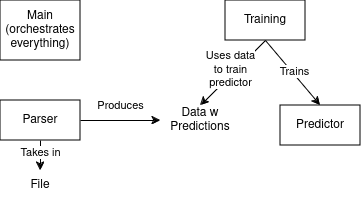
\includegraphics[width=0.5\textwidth]{task2-train-diagram.png}
\caption{Anorexia Training}
\label{FigT2Tr}
\end{figure}

\begin{figure}[H]
\centering
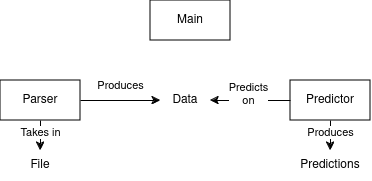
\includegraphics[width=0.5\textwidth]{task2-test.png}
\caption{Anorexia Predicting}
\label{FigT2Tes}
\end{figure}

\subsection{Eating Disorders}

The eating disorders pipeline involves the usage of a relabeling technique. This technique takes the ED data, which original only has scores for each user, and produces scores for each post. The prediction model is then trained to predict these post level scores. Then these predictions are aggregated to user level predictions which are evaluated against what the user scores should be. The rational behind this relabeling method will be explored more in the VnV report.

\begin{figure}[H]
\centering
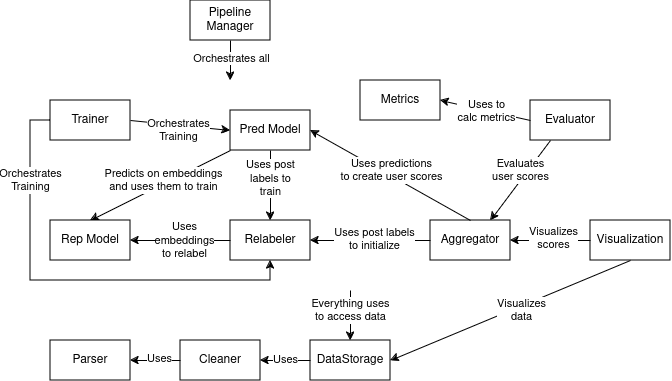
\includegraphics[width=1\textwidth]{ED-uses-diagram.png}
\caption{ED Uses Diagram}
\label{FigT3Uses}
\end{figure}

\section{Timeline}

\begin{itemize}
    \item Module: \edmref{edmPars} and \edmref{edmClean} Finish Date: Jan 20 2024 Assignee(s): Jessica
    \item Module: \edmref{edmO} Finish Date: Jan 22 2024 Assignee(s): Jessica
    \item Module: \edmref{edmData} Finish Date: Jan 26 2024 Assignee(s): Jessica
    \item Module: \edmref{edmRM} Finish Date: Jan 28 2024 Assignee(s): Jessica
    \item Module: \edmref{edmRel} Finish Date: Feb 4 2024 Assignee(s): Jessica
    \item Module: \edmref{edmPM} Finish Date: Feb 8 2024 Assignee(s): Jessica
    \item Module: \edmref{edmAgg} Finish Date: Feb 10 2024 Assignee(s): Jessica
    \item Module: \edmref{edmMets} and \edmref{edmEval} Finish Date: Feb 11 2024 Assignee(s): Jessica
    \item Module: \edmref{edmTr} Finish Date: Feb 13 2024 Assignee(s): Jessica
    \item Module: \edmref{edmPipeline} Finish Date: Feb 15 2024 Assignee(s): Jessica
    \item Module: \mref{DNOM1} Finish Date: Feb 1 2024 Assignee(s): Franklin, Matthew
    \item Module: \mref{DNOM2} Finish Date: Feb 1 2024 Assignee(s): Franklin, Matthew
    \item Module: \mref{DNOM3} Finish Date: Feb 1 2024 Assignee(s): Franklin, Matthew
    \item Module: \mref{DNOM4} Finish Date: Feb 1 2024 Assignee(s): Franklin, Matthew
    \item Module: \mref{DNOM5} Finish Date: Feb 1 2024 Assignee(s): Franklin, Matthew
    \item Module: \mref{ANOM1} Finish Date: Feb 1 2024 Assignee(s): Michael, Ben
    \item Module: \mref{ANOM2} Finish Date: Feb 1 2024 Assignee(s): Michael, Ben
    \item Module: \mref{ANOM3} Finish Date: Feb 1 2024 Assignee(s): Michael, Ben
    \item Module: \mref{ANOM4} Finish Date: Feb 1 2024 Assignee(s): Michael, Ben
    \item Module: \mref{mHH} Finish Date: Feb 1 2024 Assignee(s): All
    \item Testing (PyTest): \mref{DNOM1}, \mref{DNOM2}, \mref{DNOM3} Finish Date: Feb 2 2024 Assignee(s): Franklin, Matthew
    \item Testing (PyTest): \mref{ANOM1}, \mref{ANOM2}, \mref{ANOM3} Finish Date: Feb 2 2024 Assignee(s): Michael, Ben
    \item Testing (PyTest): \mref{DNOM4}, \mref{DNOM5} Finish Date: Feb 3 2024 Assignee(s): Franklin, Matthew
    \item Testing (PyTest): \mref{ANOM4} Finish Date: Feb 4 2024 Assignee(s): Michael, Ben
    \item Testing: All Modules Finish Date: Feb 4 2024 Assignee(s): All
\end{itemize}

%\section*{References}

\bibliographystyle {plainnat}
\bibliography{../../../refs/References}

\newpage{}

\end{document}